% Experiment 1
\subsection{Theoretical and Experimental Data}
% Tabulate all data, experimental and calculated, and include them in your report (combined with lab assignment #6)


\clearpage
\subsection{Composite Density}
% Determine the average composite density before and after cure, along with the standard deviation.  What is the average uncured thickness of each composite ply?  What is the average cured thickness of each composite ply?  How does this compare to the specifications in Table 1.2 for this composite system (for the cured ply only)?

Based on the dimensions and mass from Table \ref{tab:beforedimensions}, the densities of each specimen was tabulated in Table \ref{tab:beforedensity} assuming each specimen is a rectangular prism. The average densities and standard deviation for both uncured and cured specimens are shown as well. Table \ref{tab:ply_thickness} shows the thickness of each composite ply, where 16 plies were used to construct specimens a and b, and 8 plies were used for specimen c. This was compared to the datasheet provided from Table 1.2 in the lab manual \cite{labmanual}.

\begin{table}[!h]
    \centering
    \caption{Composite Densities}
    \begin{tabular}{|l||c|c|}\toprule
        Specimen & Uncured Density & Cured Density \\ 
        & (\textit{g / cm$^{3}$}) & (\textit{g / cm$^{3}$}) \\ \midrule
        \textbf{(a)}: $[90\degree]_{16\text{T}}$  & 1.4739 & 1.5691 \\\hline
        \textbf{(b)}: $[\pm45\degree_4]_{2\text{S}}$ & 1.4656  & 1.5667 \\\hline
        \textbf{(c)}: $[0\degree]_{8\text{T}}$ & 1.4716 & 1.5726 \\\bottomrule
        Average & 1.4703 & 1.5695 \\\hline
        Standard Deviation & 0.0043 & 0.0030 \\\bottomrule
    \end{tabular}
    \label{tab:beforedensity}
\end{table}

\begin{table}[!h]
    \centering
    \caption{Ply Thickness}
    \begin{tabular}{|l||c|c|c|}\toprule
        Specimen & Uncured Thickness & Cured Thickness & Cured Thickness \\
        & (\textit{mm}) & (\textit{mm}) & Datasheet (\textit{mm}) \\ \midrule
        \textbf{(a)}: $[90\degree]_{16\text{T}}$  & 0.1647 & 0.1383 & 0.1524 \\\hline
        \textbf{(b)}: $[\pm45\degree_4]_{2\text{S}}$ & 0.2162 & 0.1584 & 0.1524 \\\hline
        \textbf{(c)}: $[0\degree]_{8\text{T}}$ & 0.2414 & 0.1936 & 0.1524 \\\bottomrule
        Average & 0.2074 & 0.1634 & 0.1524 \\\bottomrule
    \end{tabular}
    \label{tab:ply_thickness}
\end{table}

The average cured densities for all specimens was 1.5695 g/cm$^{3}$. The datasheet predicts the average cured density for this composite should be approximately 1.53 g/cm$^{3}$. The percent difference between the experimental specimens and the datasheet density is 2.58\%, which is very similar. On the other hand, there appears to be a higher deviation between the datasheet and experimental ply thickness. The average experimental cured ply thickness was 0.1632 mm while the data sheet states the cured ply thickness is 0.1524 mm, or a 7.21\% difference. While this is fairly close to the data sheet, there are still possible explanations for this discrepancy. One possible source of this error could be manufacturing precision. Considering the specimens were constructed by hand with simple tools (scissors and rulers) and are not dimensionally exactly the same as its mold, it is likely these specimens are not constructed up to ideal specifications. For example, a varying amount of residual resin or voids could be in between each fiber, changing the distance between each ply, thus varying the ply thickness.   


\subsection{Fiber Volume Fraction}
% Using the data in Table 1.2 and question (1), and assuming zero voids in the specimens, determine the fiber volume fraction for the composite before and after cure in each specimen.  How does the cured composite fiber volume fraction compare to the material specifications?  What are possible sources of error?


\clearpage
\subsection{Volumetric Shrinkage}
% What is the total volumetric shrinkage of each composite specimen after cure?  How does this compare to the materials specification data?

Based on the dimensions of the specimen before and after curing, the volumetric shrinkage was calculated with Equation \ref{eq:volume_shrinkage}. The $V_\text{uncured}$ and $V_\text{cured}$ terms represent the volume of the specimen, uncured and cured, respectively. The shrinkage values for each specimen is shown in Table \ref{tab:volume_shrinkage_tab}. 

\begin{equation} \label{eq:volume_shrinkage}
    \% \text{Shrinkage} = \frac{V_\text{uncured} - V_\text{cured}}{V_\text{cured}} * 100 \%
\end{equation}


\begin{table}[!h]
    \centering
    \caption{Volumetric Shrinkage}
    \begin{tabular}{|l||c|c|c|}\toprule
        Specimen & Uncured Volume & Cured Volume & Shrinkage \\ 
        & (\textit{cm$^{3}$}) & (\textit{cm$^{3}$}) & (\%) \\ \midrule
        \textbf{(a)}: $[90\degree]_{16\text{T}}$ & 11.65 & 8.74 & 33.28 \\\hline
        \textbf{(b)}: $[\pm45\degree_4]_{2\text{S}}$ & 14.45 & 10.81 & 33.63 \\\hline
        \textbf{(c)}: $[0\degree]_{8\text{T}}$ & 8.28 & 6.21 & 33.40 \\\bottomrule
    \end{tabular}
    \label{tab:volume_shrinkage_tab}
\end{table}

Based on the lab manual, from Table 1.2 in Appendix G, the volumetric shrinkage is expected to be 70\%. However, from Table \ref{tab:volume_shrinkage_tab}, the experimental shrinkage was only about 33\%. Again, this is likely due to poor manufacturing tolerances. This also lines up with the theory that there are more voids or excess resin left in the composite, thus increasing the specimens' final volume and decreasing its shrinkage percentages.

\subsection{Applied Force}
% Calculate the force needed to be applied by the hot press platens to achieve 150 psi on the specimens.

In order to achieve 150 psi of pressure on the specimen, the hot press must apply a total of at least 1,050 lbf. Each specimen is 1x7 inches. By distributing the pressure evenly to all 7 sq inches, 1,050 lbf is needed. However, note that the force required is likely slightly higher since this calculation assumes the total contact area is exactly the same area as the specimen area. In reality, given all the mounting hardware and mold, the contact area must be higher than the specimen size.


\clearpage
\subsection{Post-Curing Observations}
% Comment on the quality of the manufactured specimens.  (Where there any problems during lay-up or cure which may impact the mechanical performance?)
In an ordinary semester, without the Covid-19 quarantine situation, the specimen would be removed from their molds after curing and the condition observed.  Due to state-wide shutdown, it was not possible for students to physically retrieve the specimen and observe its condition.  According to an email from Professor Ioannis Chasiotis, dated May 8, 2020, the thickness of the specimen decreased.  With this observation, the only inference possible without physical observation is that the platens have sunk deeper into the mold following the curing process.

\subsection{Specimen Cure Temperature}
% What would happen if the cure temperature was raised to a higher temperature?  How about a lower temperature?
\tab The DA 409U/G35 150 prepreg used in this experiment requires temperature cure to properly complete the manufacturing process and create the epoxy cross-links.  The temperature curing process, a process henceforth defined as thermosetting, is a very critical stage wherein temperature and pressure is applied to the specimen through a hot press to begin the polymerization, or cross-linking of the resin matrix.  In this experiment, a prepreg was used to form the specimen, which is useful for generating small, thin-skinned specimen for testing or thin walled applications, but is prone to premature curing depending on the local room temperature.

During the assembling process (\textit{lay-up stage}) of the composite specimen, an observation was made such that the curing process was able to begin prematurely due to the local heat generated by physical touch.  The lab manual warned of consequences directly linked to premature curing such as reduced mechanical quality due to malformed epoxy cross-links.  As such, rapid freezing or chilling techniques using condensed air or placement near a cold thermal-sink were applied to mitigate premature cure.  When the specimen were fully assembled, they were placed into molds (\textit{pre-cure stage}) with peeler ply, release film, and bleeder cloths.  When completed, the composites were ready for the thermosetting process.

\newpage
It is important to note that the temperature setting for the curing stage was controlled by the teaching assistants; and, variation of the curing temperature was not a focus of this experiment.  The temperature and pressure applied for the curing process was selected and performed according to the Carver programmable hot press with a cure cycle programmed by the lab staff.  If the temperature were to increase, the development of the cross-links would be much faster and rapid, which may improve the cure by preventing resin bleed and higher shrinkage would occur.  Higher shrinkage, depending on the application, may be desired due to the improvement in the material's thermal and electrical conductivity \cite{curematters}.  Higher temperature is not always good, though, as excessive temperature can result in a severe degradation of resin matrix.\cite{boeingcuring}  A lower temperature setting for the cure process of the specimen might result in the desired design performance due to a lower setting of the cross-link structures.  Variation of curing temperature may result in a variation in the quality of the cross-link structures, resin leakage, or material shrinkage.

\subsection{Specimen Cure Pressure}
% What would happen if the applied pressure was raised to a higher pressure? How about a lower pressure?

\clearpage
\subsection{Lay-up Temperature/Pressure}
% Include the average room temperature and humidity during lay-up.  Would the quality of the manufactured specimens be affected by the room temperature and humidity levels?  Explain.

The lab group did not record the average room temperature and humidity readings during the lay-up process. Thus, we presume that the the lay-up process was completed under standard lab conditions: 23$\degree$C and 40\% relative humidity. Room temperature and humidity levels are influential on the quality of manufactured specimens. During storage, the composite prepreg is kept at freezing temperatures. As the temperature increases, the epoxy will begin to crosslink. While this behavior is desired during the curing process, it is important to to avoid curing the composites prematurely from a high room temperature. Note that premature crosslinking reduces the quality of the composite specimen. It is also important to regulate the humidity level during the layup process to prevent the specimen from absorbing additional moisture. Moisture absorption can lead to the formation of more voids, which are unfilled pores in the specimen. These voids are major manufacturing defects that reduce the performance of the specimen in terms of mechanical properties and lifespan.

\subsection{Cure Cycle Temperature/Pressure History}
% Include the temperature and pressure history of the cure cycle in the report.
After the layup phase is completed, the curing process can begin. In general, the curing process involves exposing the specimen to high temperatures and pressures. Both the magnitude and duration of the elevated temperatures and pressures influence the quality of the final specimen. Different materials require different cure cycle characteristics for optimal results. A typical cure cycle can be divided in two major steps: the consolidation stage and the cure stage. During the consolidation stage, heat is applied to reach an intermediate temperature and pressure is applied. The heat reduces the viscosity of the resin and the pressure squeezes excess resin out of the laminate. The pressure also "consolidates" the individual specimen plies and removes voids.  During the cure stage, the temperature is elevated even more. The higher temperature initiates resin polymerization and produces cross-linking. 

\begin{figure}[H]
    \centering
    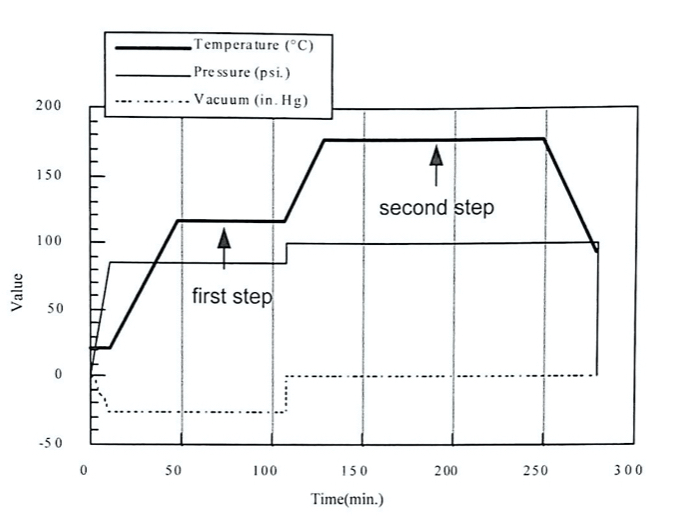
\includegraphics[width=0.8\textwidth]{Pictures/Lab1: Q 1.10/typical_cure.jpg}
    \caption{Typical Cure Cycle\cite{labmanual}}
    \label{fig:typicalcure}
\end{figure}

Figure \ref{fig:typicalcure} displays the temperatures and pressures in a typical cure cycle. Here, the difference in temperatures and pressures between the first and second steps can be seen. Note that this figure corresponds to a typical cure cycle, and not the one used for this lab.

For this lab, a single step cure cycle is used. In this case, the temperature and pressure are raised to a predetermined value only once. Figure \ref{fig:mariecuring} displays the curing cycle for the specimen used in this lab. The single step, as opposed to two steps in the cycle discussed earlier, can be seen in this figure.



% \clearpage
\subsection{Cure Cycle Heating/Cooling Rate}
% Explain why the heating rate is much more linear than the cooling rate.

The curing cycle involves a rise in temperature for polymerization and then a cooling period afterwards. The temperatures that the specimen experiences during the cycle are determined by the hot press platens. It is important to note that the platens do not heat and cool at the same rate. The heating rate is much more linear than the cooling rate, which can be attributed to the processes by which the platens are heated and cooled. The heating rate is controlled through a process known as Joule heating. In this process, an electrical current is passed through a conductor, which produces heat. The heating rate can then be monitored using a thermocouple and actively controlled through the electric current. In contrast, the platens are cooled using flowing chilled water. In this case, not only is the cooling rate not actively controlled, but the flow rate is also constant. The cooling rate of the platens slows down over time since the temperature of the platens decreases, while the temperature of the chilled flowing water is constant. This results in a nonlinear cooling rate.

\subsection{Cure Cycle Compaction}
% When does compaction of the composite laminate take place during the cure cycle? (Hint: When does the platen height change dramatically during the cure cycle?)


% Experiment 6
% \setcounter{subsection}{0} % ONLY FOR DEBUGGING PURPOSES


\subsection{Stress and Strain Curves}
% Plot the stress versus strain curves for each test using the strain from the digital extensometer and the DIC calculations (i.e. two curves for each specimen).  Plot both stress vs strain curves for each specimen in the same plot.

In order to get an accurate idea of how these materials behaved and the mechanical properties of each layup, a stress vs. strain graph is a very useful tool. In this experiment the strain on each specimen was measured using two different methods, a digital image correlation (DIC) and the Instrom 2630-100 digital extensometer. This allowed for more accurate measurements to be taken and then compared once the experiment was finished. Although, there was an offset from between the DIC and extensometer, so that had to be corrected in the data before an accurate comparison could take place. With information on the strain, load, and size of each specimen, the following figures could be created for the $0\degree$, $45\degree$, and $90\degree$ laminates shown in Fig \ref{fig:stressvsstrain}.  One interesting to note from this is the behavior before breaking of all three tests. It can be seen in Fig \ref{fig:0lam} and Fig \ref{fig:90lam} that the stress is fairly linear until there is a sudden catastrophic failure with very little deformation of the material. This has to do with the orientation of the ply's within the composite, and when the are either parallel or perpendicular to the force, this type of behavior is to be expected. In Fig \ref{fig:45lam}, there is a linear region that translates to a more shallow slope until failure. This type of behavior occurs again due to the orientation of the laminates, with the load being distributed through both the matrix and fibers of the composite resulting in greater deformation and changes in the material property before failure. 

\begin{figure}[!h]
    \begin{center}
    \begin{subfigure}[b]{0.45\linewidth}
        \centering
        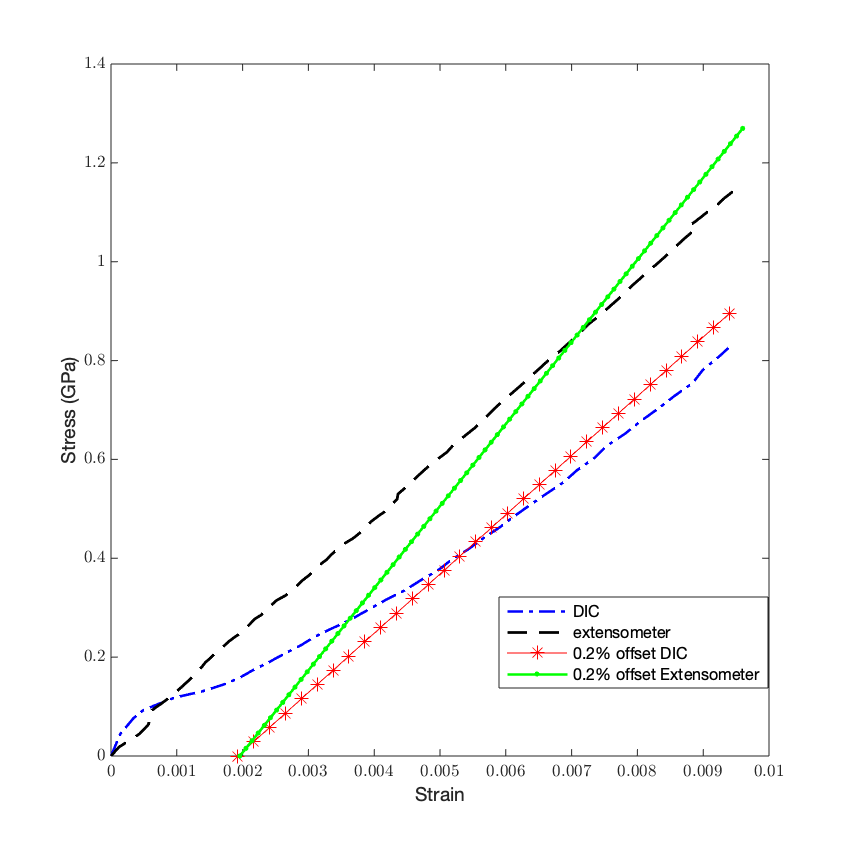
\includegraphics[width=\linewidth]{Pictures/stress vs strain/StressvsStrain_0.png}
        \caption{\textbf 0$\degree$ laminate}
        \label{fig:0lam}
    \end{subfigure}
    \begin{subfigure}[b]{0.45\linewidth}
        \centering
        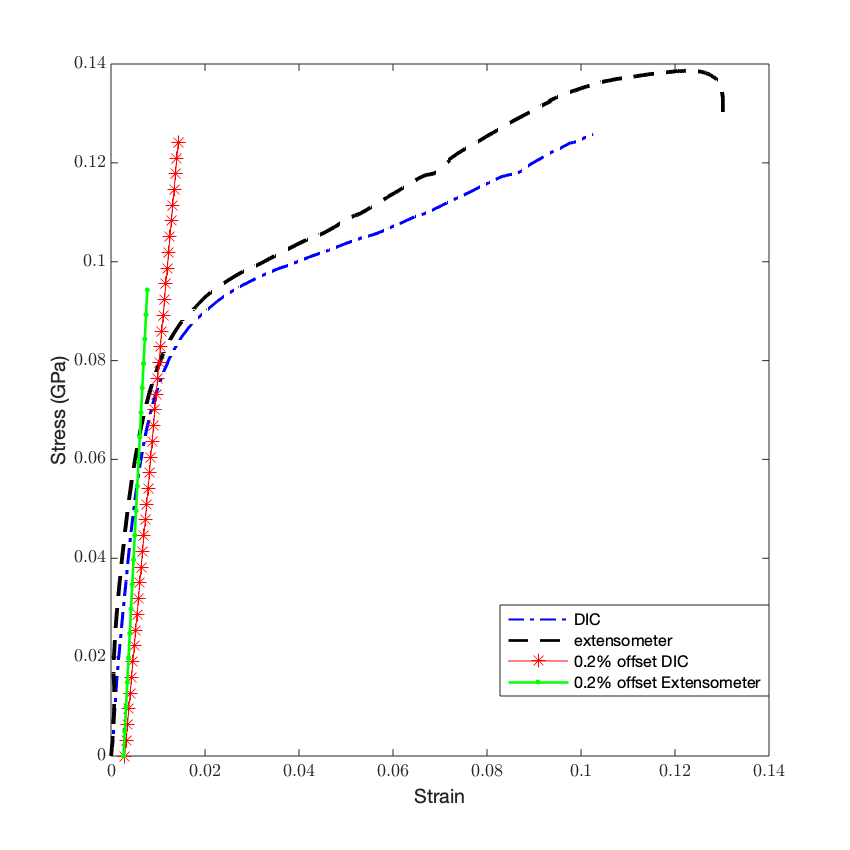
\includegraphics[width=\linewidth]{Pictures/stress vs strain/StressvsStrain_45.png}
        \caption{\textbf 45$\degree$ laminate}
        \label{fig:45lam}
    \end{subfigure}
    \end{center}
    \begin{center}
    \begin{subfigure}[b]{0.45\linewidth}
        \centering
        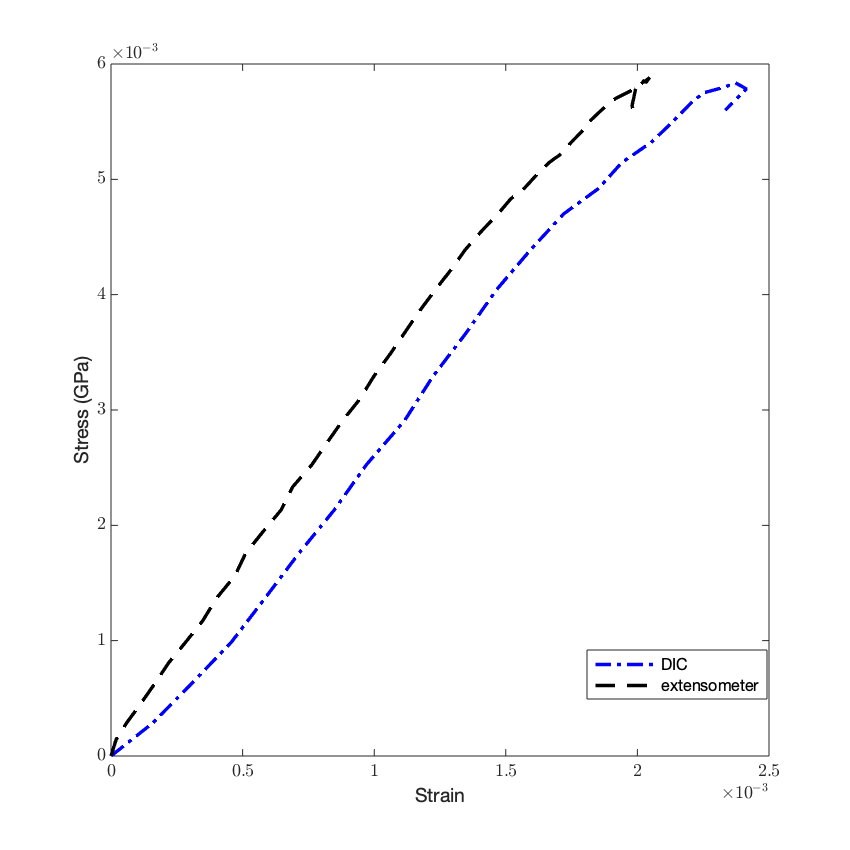
\includegraphics[width=\linewidth]{Pictures/stress vs strain/StressvsStrain_90.png}
        \caption{\textbf 90$\degree$ laminate}
        \label{fig:90lam}
    \end{subfigure}
    \end{center}
    \caption{Stress vs Strain plots comparing DIC to Extensometer measurements}
    \label{fig:stressvsstrain}
\end{figure}

\subsection{Specimen Experimental Values}
% Obtain experimental values of elastic modulus, elastic limit, ultimate strength, and ultimate strain for each specimen using the strain from the digital extensometer and the DIC calculations.  Tabulate all data and present them in your write-up.


% \clearpage
\subsection{Theoretical On and Off-axis Composite Properties}
% Compute all on-axis and off-axis composite properties using the micromechanics models found in equations (6.8)-(6.11), (6.23)(6.27), and (6.28)-(6.33).
N

% \clearpage
\subsection{Theoretical Effective Composite Properties}
% Compute the theoretical properties (E1, E2, nu12, and G6) for each composite specimen using equations (6.20) and (6.34)-(6.38).
N

\clearpage
\subsection{Experimental Modulus}
% Compare the experimental modulus (E1) for the composite specimens (as measured with the digital extensometer and from your DIC calculations) and the predictions determined in (4).

\begin{table}[!h]
    \centering
    \caption{Comparison of E$_{1}$ \cite{labmanual}}
    \begin{tabular}{|C{1in}|c|c|c|}\toprule
        \multicolumn{4}{c}{\textbf{Theoretical and Experimental Modulus}} \\ \midrule
        \textbf{Laminate\newline Orientation} & \textbf{Theoretical} & \textbf{DIC} & \textbf{Extensometer} \\ \hline\hline
         $0\degree$ & 130.37 GPa & 119.84 GPa & 166 GPa \\\hline
        $45\degree$ & 5.918 GPa & 10.9 GPa & 18 GPa  \\\hline
        $90\degree$ & 5.484 GPa & 2.69 GPa & 2.59 GPa \\\bottomrule
    \end{tabular}
    \label{tab:e1}
\end{table}

Compared to the theoretical values, the experimental modulus from DIC is lower for the $0\degree$ and $90\degree$ laminate orientations but greater for the $45\degree$ orientation. The experimental modulus from the extensometer is larger than the other results for both the $0\degree$ and $45\degree$ specimens but is the lowest for the $90\degree$ orientation.

% \clearpage
\subsection{Failure Loads}
% Compute the theoretical failure loads of the 0 deg and 90 deg composite specimens using equation (6.54). Compute the failure load for the off-axis +/-45 deg composite specimen using the same equation (Hint: Assume theta = +45 deg only).  Compare these results with those obtained experimentally.
\begin{table}[!h]
    \centering
    \caption{Theoretical and Experimental Tensile Failure Loads \cite{labmanual}}
    \begin{tabular}{|C{1in}|c|c|}\toprule
        \multicolumn{3}{c}{\textbf{Tensile Failure Loads}} \\ \midrule
        \textbf{Laminate\newline Orientation} & \textbf{Theoretical} & \textbf{Experimental} \\ \hline\hline
        $0\degree$  & 1.930 GPa  & 1.156 GPa \\\hline
        $45\degree$ & 0.0668 GPa & 0.1386 GPa \\\hline
        $90\degree$ & 0.040 GPa  & 0.0059 GPa \\\bottomrule
    \end{tabular}
    \label{tab:failureloads}
\end{table}

The experimental failure loads are lower for the $0\degree$ and $90\degree$ laminate orientations. However, the experimental failure load is higher for the $45\degree$ specimen. 



\clearpage
\subsection{Specific Elastic Modulus and Strength}
% Compute the specific elastic modulus and specific strength of all the specimens using the composite density data generated for each cured specimen in the manufacturing lab, Lab #1.  Compare the values of the three specimens to each another.
\begin{table}[!h]
    \centering
    \caption{Specimen specific properties \cite{labmanual}}
    \begin{tabular}{|C{1in}|c|c|}\toprule
        \multicolumn{3}{c}{\textbf{Specific Properties}} \\ \midrule
        \textbf{Laminate\newline Orientation} & \textbf{Specific Elastic Modulus} & \textbf{Specific Strength} \\ \hline\hline
         $0\degree$ & 76.21 MPa  & 735.1 $\frac{kPa}{kg/m^{3}}$ \\\hline
        $45\degree$ & 6.957 MPa & 88.49 $\frac{kPa}{kg/m^{3}}$  \\\hline
        $90\degree$ & 1.714 MPa & 3.749 $\frac{kPa}{kg/m^{3}}$  \\\bottomrule
    \end{tabular}
    \label{tab:specprop}
\end{table}

The specific elastic modulus and specific strength of the $0\degree$ laminate orientation specimen is much greater than the other two orientations. Even so, the $45\degree$ specimen still has significantly greater specific elastic modulus and specific strength than the $90\degree$ orientation.

\subsection{Theoretical and Experimental Disparities}
% Comment on any disparities between model predictions and experimental values.  What are possible causes of discrepancies?